\documentclass[1p]{elsarticle_modified}
%\bibliographystyle{elsarticle-num}

%\usepackage[colorlinks]{hyperref}
%\usepackage{abbrmath_seonhwa} %\Abb, \Ascr, \Acal ,\Abf, \Afrak
\usepackage{amsfonts}
\usepackage{amssymb}
\usepackage{amsmath}
\usepackage{amsthm}
\usepackage{scalefnt}
\usepackage{amsbsy}
\usepackage{kotex}
\usepackage{caption}
\usepackage{subfig}
\usepackage{color}
\usepackage{graphicx}
\usepackage{xcolor} %% white, black, red, green, blue, cyan, magenta, yellow
\usepackage{float}
\usepackage{setspace}
\usepackage{hyperref}

\usepackage{tikz}
\usetikzlibrary{arrows}

\usepackage{multirow}
\usepackage{array} % fixed length table
\usepackage{hhline}

%%%%%%%%%%%%%%%%%%%%%
\makeatletter
\renewcommand*\env@matrix[1][\arraystretch]{%
	\edef\arraystretch{#1}%
	\hskip -\arraycolsep
	\let\@ifnextchar\new@ifnextchar
	\array{*\c@MaxMatrixCols c}}
\makeatother %https://tex.stackexchange.com/questions/14071/how-can-i-increase-the-line-spacing-in-a-matrix
%%%%%%%%%%%%%%%

\usepackage[normalem]{ulem}

\newcommand{\msout}[1]{\ifmmode\text{\sout{\ensuremath{#1}}}\else\sout{#1}\fi}
%SOURCE: \msout is \stkout macro in https://tex.stackexchange.com/questions/20609/strikeout-in-math-mode

\newcommand{\cancel}[1]{
	\ifmmode
	{\color{red}\msout{#1}}
	\else
	{\color{red}\sout{#1}}
	\fi
}

\newcommand{\add}[1]{
	{\color{blue}\uwave{#1}}
}

\newcommand{\replace}[2]{
	\ifmmode
	{\color{red}\msout{#1}}{\color{blue}\uwave{#2}}
	\else
	{\color{red}\sout{#1}}{\color{blue}\uwave{#2}}
	\fi
}

\newcommand{\Sol}{\mathcal{S}} %segment
\newcommand{\D}{D} %diagram
\newcommand{\A}{\mathcal{A}} %arc


%%%%%%%%%%%%%%%%%%%%%%%%%%%%%5 test

\def\sl{\operatorname{\textup{SL}}(2,\Cbb)}
\def\psl{\operatorname{\textup{PSL}}(2,\Cbb)}
\def\quan{\mkern 1mu \triangleright \mkern 1mu}

\theoremstyle{definition}
\newtheorem{thm}{Theorem}[section]
\newtheorem{prop}[thm]{Proposition}
\newtheorem{lem}[thm]{Lemma}
\newtheorem{ques}[thm]{Question}
\newtheorem{cor}[thm]{Corollary}
\newtheorem{defn}[thm]{Definition}
\newtheorem{exam}[thm]{Example}
\newtheorem{rmk}[thm]{Remark}
\newtheorem{alg}[thm]{Algorithm}

\newcommand{\I}{\sqrt{-1}}
\begin{document}

%\begin{frontmatter}
%
%\title{Boundary parabolic representations of knots up to 8 crossings}
%
%%% Group authors per affiliation:
%\author{Yunhi Cho} 
%\address{Department of Mathematics, University of Seoul, Seoul, Korea}
%\ead{yhcho@uos.ac.kr}
%
%
%\author{Seonhwa Kim} %\fnref{s_kim}}
%\address{Center for Geometry and Physics, Institute for Basic Science, Pohang, 37673, Korea}
%\ead{ryeona17@ibs.re.kr}
%
%\author{Hyuk Kim}
%\address{Department of Mathematical Sciences, Seoul National University, Seoul 08826, Korea}
%\ead{hyukkim@snu.ac.kr}
%
%\author{Seokbeom Yoon}
%\address{Department of Mathematical Sciences, Seoul National University, Seoul, 08826,  Korea}
%\ead{sbyoon15@snu.ac.kr}
%
%\begin{abstract}
%We find all boundary parabolic representation of knots up to 8 crossings.
%
%\end{abstract}
%\begin{keyword}
%    \MSC[2010] 57M25 
%\end{keyword}
%
%\end{frontmatter}

%\linenumbers
%\tableofcontents
%
\newcommand\colored[1]{\textcolor{white}{\rule[-0.35ex]{0.8em}{1.4ex}}\kern-0.8em\color{red} #1}%
%\newcommand\colored[1]{\textcolor{white}{ #1}\kern-2.17ex	\textcolor{white}{ #1}\kern-1.81ex	\textcolor{white}{ #1}\kern-2.15ex\color{red}#1	}

{\Large $\underline{12a_{1093}~(K12a_{1093})}$}

\setlength{\tabcolsep}{10pt}
\renewcommand{\arraystretch}{1.6}
\vspace{1cm}\begin{tabular}{m{100pt}>{\centering\arraybackslash}m{274pt}}
\multirow{5}{120pt}{
	\centering
	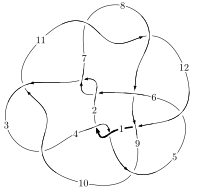
\includegraphics[width=112pt]{../../../GIT/diagram.site/Diagrams/png/1894_12a_1093.png}\\
\ \ \ A knot diagram\footnotemark}&
\allowdisplaybreaks
\textbf{Linearized knot diagam} \\
\cline{2-2}
 &
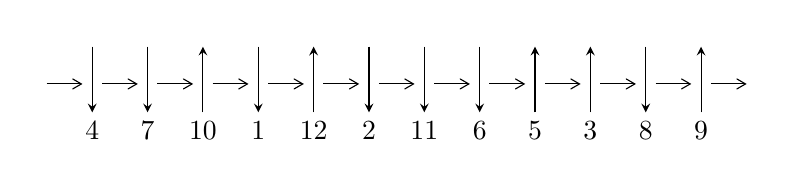
\begin{tikzpicture}[x=20pt, y=17pt]
	% nodes
	\node (C0) at (0, 0) {};
	\node (C1) at (1, 0) {};
	\node (C1U) at (1, +1) {};
	\node (C1D) at (1, -1) {4};

	\node (C2) at (2, 0) {};
	\node (C2U) at (2, +1) {};
	\node (C2D) at (2, -1) {7};

	\node (C3) at (3, 0) {};
	\node (C3U) at (3, +1) {};
	\node (C3D) at (3, -1) {10};

	\node (C4) at (4, 0) {};
	\node (C4U) at (4, +1) {};
	\node (C4D) at (4, -1) {1};

	\node (C5) at (5, 0) {};
	\node (C5U) at (5, +1) {};
	\node (C5D) at (5, -1) {12};

	\node (C6) at (6, 0) {};
	\node (C6U) at (6, +1) {};
	\node (C6D) at (6, -1) {2};

	\node (C7) at (7, 0) {};
	\node (C7U) at (7, +1) {};
	\node (C7D) at (7, -1) {11};

	\node (C8) at (8, 0) {};
	\node (C8U) at (8, +1) {};
	\node (C8D) at (8, -1) {6};

	\node (C9) at (9, 0) {};
	\node (C9U) at (9, +1) {};
	\node (C9D) at (9, -1) {5};

	\node (C10) at (10, 0) {};
	\node (C10U) at (10, +1) {};
	\node (C10D) at (10, -1) {3};

	\node (C11) at (11, 0) {};
	\node (C11U) at (11, +1) {};
	\node (C11D) at (11, -1) {8};

	\node (C12) at (12, 0) {};
	\node (C12U) at (12, +1) {};
	\node (C12D) at (12, -1) {9};
	\node (C13) at (13, 0) {};

	% arrows
	\draw[->,>={angle 60}]
	(C0) edge (C1) (C1) edge (C2) (C2) edge (C3) (C3) edge (C4) (C4) edge (C5) (C5) edge (C6) (C6) edge (C7) (C7) edge (C8) (C8) edge (C9) (C9) edge (C10) (C10) edge (C11) (C11) edge (C12) (C12) edge (C13) ;	\draw[->,>=stealth]
	(C1U) edge (C1D) (C2U) edge (C2D) (C3D) edge (C3U) (C4U) edge (C4D) (C5D) edge (C5U) (C6U) edge (C6D) (C7U) edge (C7D) (C8U) edge (C8D) (C9D) edge (C9U) (C10D) edge (C10U) (C11U) edge (C11D) (C12D) edge (C12U) ;
	\end{tikzpicture} \\
\hhline{~~} \\& 
\textbf{Solving Sequence} \\ \cline{2-2} 
 &
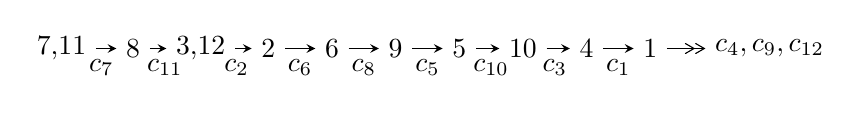
\begin{tikzpicture}[x=23pt, y=7pt]
	% node
	\node (A0) at (-1/8, 0) {7,11};
	\node (A1) at (1, 0) {8};
	\node (A2) at (33/16, 0) {3,12};
	\node (A3) at (25/8, 0) {2};
	\node (A4) at (33/8, 0) {6};
	\node (A5) at (41/8, 0) {9};
	\node (A6) at (49/8, 0) {5};
	\node (A7) at (57/8, 0) {10};
	\node (A8) at (65/8, 0) {4};
	\node (A9) at (73/8, 0) {1};
	\node (C1) at (1/2, -1) {$c_{7}$};
	\node (C2) at (3/2, -1) {$c_{11}$};
	\node (C3) at (21/8, -1) {$c_{2}$};
	\node (C4) at (29/8, -1) {$c_{6}$};
	\node (C5) at (37/8, -1) {$c_{8}$};
	\node (C6) at (45/8, -1) {$c_{5}$};
	\node (C7) at (53/8, -1) {$c_{10}$};
	\node (C8) at (61/8, -1) {$c_{3}$};
	\node (C9) at (69/8, -1) {$c_{1}$};
	\node (A10) at (11, 0) {$c_{4},c_{9},c_{12}$};

	% edge
	\draw[->,>=stealth]	
	(A0) edge (A1) (A1) edge (A2) (A2) edge (A3) (A3) edge (A4) (A4) edge (A5) (A5) edge (A6) (A6) edge (A7) (A7) edge (A8) (A8) edge (A9) ;
	\draw[->>,>={angle 60}]	
	(A9) edge (A10);
\end{tikzpicture} \\ 

\end{tabular} \\

\footnotetext{
The image of knot diagram is generated by the software ``\textbf{Draw programme}" developed by Andrew Bartholomew(\url{http://www.layer8.co.uk/maths/draw/index.htm\#Running-draw}), where we modified some parts for our purpose(\url{https://github.com/CATsTAILs/LinksPainter}).
}\phantom \\ \newline 
\centering \textbf{Ideals for irreducible components\footnotemark of $X_{\text{par}}$} 
 
\begin{align*}
I^u_{1}&=\langle 
2.41694\times10^{695} u^{134}+4.64040\times10^{695} u^{133}+\cdots+5.96213\times10^{699} b-1.44042\times10^{700},\\
\phantom{I^u_{1}}&\phantom{= \langle  }-1.38922\times10^{698} u^{134}-1.25918\times10^{698} u^{133}+\cdots+3.78595\times10^{701} a+4.01348\times10^{701},\\
\phantom{I^u_{1}}&\phantom{= \langle  }u^{135}+u^{134}+\cdots-29624 u+4064\rangle \\
I^u_{2}&=\langle 
-8.63325\times10^{19} u^{27}-6.49290\times10^{20} u^{26}+\cdots+3.25555\times10^{19} b+1.08679\times10^{21},\\
\phantom{I^u_{2}}&\phantom{= \langle  }2.39039\times10^{20} u^{27}+1.89818\times10^{21} u^{26}+\cdots+6.51111\times10^{19} a-4.16427\times10^{21},\;u^{28}+8 u^{27}+\cdots-8 u+8\rangle \\
I^u_{3}&=\langle 
-4 a^3+4 a^2+3 b-3 a+1,\;4 a^4+5 a^2+2 a+2,\;u-1\rangle \\
\\
\end{align*}
\raggedright * 3 irreducible components of $\dim_{\mathbb{C}}=0$, with total 167 representations.\\
\footnotetext{All coefficients of polynomials are rational numbers. But the coefficients are sometimes approximated in decimal forms when there is not enough margin.}
\newpage
\renewcommand{\arraystretch}{1}
\centering \section*{I. $I^u_{1}= \langle 2.42\times10^{695} u^{134}+4.64\times10^{695} u^{133}+\cdots+5.96\times10^{699} b-1.44\times10^{700},\;-1.39\times10^{698} u^{134}-1.26\times10^{698} u^{133}+\cdots+3.79\times10^{701} a+4.01\times10^{701},\;u^{135}+u^{134}+\cdots-29624 u+4064 \rangle$}
\flushleft \textbf{(i) Arc colorings}\\
\begin{tabular}{m{7pt} m{180pt} m{7pt} m{180pt} }
\flushright $a_{7}=$&$\begin{pmatrix}1\\0\end{pmatrix}$ \\
\flushright $a_{11}=$&$\begin{pmatrix}0\\u\end{pmatrix}$ \\
\flushright $a_{8}=$&$\begin{pmatrix}1\\u^2\end{pmatrix}$ \\
\flushright $a_{3}=$&$\begin{pmatrix}0.000366942 u^{134}+0.000332594 u^{133}+\cdots+67.1416 u-1.06010\\-0.0000405383 u^{134}-0.0000778313 u^{133}+\cdots-19.1811 u+2.41594\end{pmatrix}$ \\
\flushright $a_{12}=$&$\begin{pmatrix}- u\\- u^3+u\end{pmatrix}$ \\
\flushright $a_{2}=$&$\begin{pmatrix}0.000326403 u^{134}+0.000254762 u^{133}+\cdots+47.9605 u+1.35585\\-0.0000405383 u^{134}-0.0000778313 u^{133}+\cdots-19.1811 u+2.41594\end{pmatrix}$ \\
\flushright $a_{6}=$&$\begin{pmatrix}-0.000256986 u^{134}-0.000372603 u^{133}+\cdots+73.1449 u-10.7816\\0.0000667386 u^{134}-5.85205\times10^{-7} u^{133}+\cdots+24.5301 u-1.64608\end{pmatrix}$ \\
\flushright $a_{9}=$&$\begin{pmatrix}-0.000634464 u^{134}-0.000889132 u^{133}+\cdots-14.6902 u-1.26794\\-0.0000357046 u^{134}-0.0000865215 u^{133}+\cdots+13.6147 u-1.72538\end{pmatrix}$ \\
\flushright $a_{5}=$&$\begin{pmatrix}-0.000272618 u^{134}-0.000395365 u^{133}+\cdots+75.5210 u-11.1880\\0.0000860364 u^{134}+0.0000347660 u^{133}+\cdots+22.0063 u-1.21078\end{pmatrix}$ \\
\flushright $a_{10}=$&$\begin{pmatrix}0.0000129880 u^{134}-0.000201145 u^{133}+\cdots-28.4490 u+8.78419\\-0.0000482932 u^{134}-0.0000371033 u^{133}+\cdots-18.7256 u+1.31562\end{pmatrix}$ \\
\flushright $a_{4}=$&$\begin{pmatrix}-0.000237685 u^{134}-0.000772866 u^{133}+\cdots-36.2106 u+10.8885\\-0.0000422265 u^{134}-0.0000873001 u^{133}+\cdots-19.4457 u+1.18457\end{pmatrix}$ \\
\flushright $a_{1}=$&$\begin{pmatrix}-0.000761097 u^{134}-0.00188751 u^{133}+\cdots-32.2015 u+9.78192\\-0.000255375 u^{134}-0.000516647 u^{133}+\cdots-21.9195 u+3.00457\end{pmatrix}$\\&\end{tabular}
\flushleft \textbf{(ii) Obstruction class $= -1$}\\~\\
\flushleft \textbf{(iii) Cusp Shapes $= 0.000378821 u^{134}+0.000233338 u^{133}+\cdots+121.501 u-5.44603$}\\~\\
\newpage\renewcommand{\arraystretch}{1}
\flushleft \textbf{(iv) u-Polynomials at the component}\newline \\
\begin{tabular}{m{50pt}|m{274pt}}
Crossings & \hspace{64pt}u-Polynomials at each crossing \\
\hline $$\begin{aligned}c_{1},c_{4}\end{aligned}$$&$\begin{aligned}
&u^{135}-9 u^{134}+\cdots+167083 u+63886
\end{aligned}$\\
\hline $$\begin{aligned}c_{2},c_{6}\end{aligned}$$&$\begin{aligned}
&u^{135}- u^{134}+\cdots+144633 u+4946
\end{aligned}$\\
\hline $$\begin{aligned}c_{3},c_{10}\end{aligned}$$&$\begin{aligned}
&4(4 u^{135}+36 u^{134}+\cdots+2779214 u+127574)
\end{aligned}$\\
\hline $$\begin{aligned}c_{5}\end{aligned}$$&$\begin{aligned}
&u^{135}-3 u^{134}+\cdots+45913 u+3188
\end{aligned}$\\
\hline $$\begin{aligned}c_{7},c_{11}\end{aligned}$$&$\begin{aligned}
&u^{135}- u^{134}+\cdots-29624 u-4064
\end{aligned}$\\
\hline $$\begin{aligned}c_{8}\end{aligned}$$&$\begin{aligned}
&4(4 u^{135}-56 u^{134}+\cdots+23579 u-1798)
\end{aligned}$\\
\hline $$\begin{aligned}c_{9}\end{aligned}$$&$\begin{aligned}
&u^{135}-3 u^{134}+\cdots+48 u+16
\end{aligned}$\\
\hline $$\begin{aligned}c_{12}\end{aligned}$$&$\begin{aligned}
&4(4 u^{135}+8 u^{134}+\cdots-21656 u-7442)
\end{aligned}$\\
\hline
\end{tabular}\\~\\
\newpage\renewcommand{\arraystretch}{1}
\flushleft \textbf{(v) Riley Polynomials at the component}\newline \\
\begin{tabular}{m{50pt}|m{274pt}}
Crossings & \hspace{64pt}Riley Polynomials at each crossing \\
\hline $$\begin{aligned}c_{1},c_{4}\end{aligned}$$&$\begin{aligned}
&y^{135}+83 y^{134}+\cdots-6695683735 y-4081420996
\end{aligned}$\\
\hline $$\begin{aligned}c_{2},c_{6}\end{aligned}$$&$\begin{aligned}
&y^{135}-93 y^{134}+\cdots-1498427007 y-24462916
\end{aligned}$\\
\hline $$\begin{aligned}c_{3},c_{10}\end{aligned}$$&$\begin{aligned}
&16(16 y^{135}+1560 y^{134}+\cdots+6.92965\times10^{11} y-1.62751\times10^{10})
\end{aligned}$\\
\hline $$\begin{aligned}c_{5}\end{aligned}$$&$\begin{aligned}
&y^{135}+23 y^{134}+\cdots-394825095 y-10163344
\end{aligned}$\\
\hline $$\begin{aligned}c_{7},c_{11}\end{aligned}$$&$\begin{aligned}
&y^{135}-119 y^{134}+\cdots-1894424256 y-16516096
\end{aligned}$\\
\hline $$\begin{aligned}c_{8}\end{aligned}$$&$\begin{aligned}
&16(16 y^{135}-568 y^{134}+\cdots+1426485 y-3232804)
\end{aligned}$\\
\hline $$\begin{aligned}c_{9}\end{aligned}$$&$\begin{aligned}
&y^{135}-11 y^{134}+\cdots-9664 y-256
\end{aligned}$\\
\hline $$\begin{aligned}c_{12}\end{aligned}$$&$\begin{aligned}
&16(16 y^{135}-248 y^{134}+\cdots+3.86816\times10^{9} y-5.53834\times10^{7})
\end{aligned}$\\
\hline
\end{tabular}\\~\\
\newpage\flushleft \textbf{(vi) Complex Volumes and Cusp Shapes}
$$\begin{array}{c|c|c}  
\text{Solutions to }I^u_{1}& \I (\text{vol} + \sqrt{-1}CS) & \text{Cusp shape}\\
 \hline 
\begin{aligned}
u &= \phantom{-}1.042300 + 0.173887 I \\
a &= \phantom{-}0.346749 + 0.407337 I \\
b &= -0.307688 + 0.981724 I\end{aligned}
 & \phantom{-}1.69401 + 1.01081 I & \phantom{-0.000000 } 0 \\ \hline\begin{aligned}
u &= \phantom{-}1.042300 - 0.173887 I \\
a &= \phantom{-}0.346749 - 0.407337 I \\
b &= -0.307688 - 0.981724 I\end{aligned}
 & \phantom{-}1.69401 - 1.01081 I & \phantom{-0.000000 } 0 \\ \hline\begin{aligned}
u &= \phantom{-}0.375168 + 0.842996 I \\
a &= -1.168620 - 0.783699 I \\
b &= \phantom{-}1.266540 + 0.437731 I\end{aligned}
 & -0.31064 - 4.93968 I & \phantom{-0.000000 } 0 \\ \hline\begin{aligned}
u &= \phantom{-}0.375168 - 0.842996 I \\
a &= -1.168620 + 0.783699 I \\
b &= \phantom{-}1.266540 - 0.437731 I\end{aligned}
 & -0.31064 + 4.93968 I & \phantom{-0.000000 } 0 \\ \hline\begin{aligned}
u &= \phantom{-}1.022720 + 0.353185 I \\
a &= -0.572973 - 0.159218 I \\
b &= \phantom{-}0.0470834 - 0.0646180 I\end{aligned}
 & -1.88121 - 1.43775 I & \phantom{-0.000000 } 0 \\ \hline\begin{aligned}
u &= \phantom{-}1.022720 - 0.353185 I \\
a &= -0.572973 + 0.159218 I \\
b &= \phantom{-}0.0470834 + 0.0646180 I\end{aligned}
 & -1.88121 + 1.43775 I & \phantom{-0.000000 } 0 \\ \hline\begin{aligned}
u &= \phantom{-}0.354628 + 0.844423 I \\
a &= \phantom{-}1.000250 + 0.197229 I \\
b &= -1.235060 - 0.186530 I\end{aligned}
 & -1.62494 - 3.37205 I & \phantom{-0.000000 } 0 \\ \hline\begin{aligned}
u &= \phantom{-}0.354628 - 0.844423 I \\
a &= \phantom{-}1.000250 - 0.197229 I \\
b &= -1.235060 + 0.186530 I\end{aligned}
 & -1.62494 + 3.37205 I & \phantom{-0.000000 } 0 \\ \hline\begin{aligned}
u &= \phantom{-}0.196400 + 0.873449 I \\
a &= \phantom{-}0.010733 + 0.241199 I \\
b &= -0.929415 - 0.243228 I\end{aligned}
 & -1.17539 - 3.86755 I & \phantom{-0.000000 } 0 \\ \hline\begin{aligned}
u &= \phantom{-}0.196400 - 0.873449 I \\
a &= \phantom{-}0.010733 - 0.241199 I \\
b &= -0.929415 + 0.243228 I\end{aligned}
 & -1.17539 + 3.86755 I & \phantom{-0.000000 } 0\\
 \hline 
 \end{array}$$\newpage$$\begin{array}{c|c|c}  
\text{Solutions to }I^u_{1}& \I (\text{vol} + \sqrt{-1}CS) & \text{Cusp shape}\\
 \hline 
\begin{aligned}
u &= -0.801867 + 0.367668 I \\
a &= \phantom{-}0.412833 + 0.031474 I \\
b &= -0.442433 - 0.840044 I\end{aligned}
 & \phantom{-}3.52686 + 1.14515 I & \phantom{-0.000000 } 0 \\ \hline\begin{aligned}
u &= -0.801867 - 0.367668 I \\
a &= \phantom{-}0.412833 - 0.031474 I \\
b &= -0.442433 + 0.840044 I\end{aligned}
 & \phantom{-}3.52686 - 1.14515 I & \phantom{-0.000000 } 0 \\ \hline\begin{aligned}
u &= \phantom{-}1.111190 + 0.197400 I \\
a &= \phantom{-}0.480641 - 0.738811 I \\
b &= \phantom{-}0.182267 + 0.083453 I\end{aligned}
 & -0.360365 + 0.099354 I & \phantom{-0.000000 } 0 \\ \hline\begin{aligned}
u &= \phantom{-}1.111190 - 0.197400 I \\
a &= \phantom{-}0.480641 + 0.738811 I \\
b &= \phantom{-}0.182267 - 0.083453 I\end{aligned}
 & -0.360365 - 0.099354 I & \phantom{-0.000000 } 0 \\ \hline\begin{aligned}
u &= \phantom{-}0.022742 + 1.129890 I \\
a &= -1.182390 + 0.135167 I \\
b &= \phantom{-}1.228750 - 0.290479 I\end{aligned}
 & -0.54814 + 5.33540 I & \phantom{-0.000000 } 0 \\ \hline\begin{aligned}
u &= \phantom{-}0.022742 - 1.129890 I \\
a &= -1.182390 - 0.135167 I \\
b &= \phantom{-}1.228750 + 0.290479 I\end{aligned}
 & -0.54814 - 5.33540 I & \phantom{-0.000000 } 0 \\ \hline\begin{aligned}
u &= -0.159127 + 0.855147 I \\
a &= -0.227634 + 1.081360 I \\
b &= \phantom{-}0.498582 - 0.643015 I\end{aligned}
 & \phantom{-}4.39896 - 3.63479 I & \phantom{-0.000000 } 0 \\ \hline\begin{aligned}
u &= -0.159127 - 0.855147 I \\
a &= -0.227634 - 1.081360 I \\
b &= \phantom{-}0.498582 + 0.643015 I\end{aligned}
 & \phantom{-}4.39896 + 3.63479 I & \phantom{-0.000000 } 0 \\ \hline\begin{aligned}
u &= -1.13139\phantom{ +0.000000I} \\
a &= \phantom{-}0.635787\phantom{ +0.000000I} \\
b &= \phantom{-}1.35448\phantom{ +0.000000I}\end{aligned}
 & -3.56663\phantom{ +0.000000I} & \phantom{-0.000000 } 0 \\ \hline\begin{aligned}
u &= -1.048410 + 0.435361 I \\
a &= \phantom{-}0.206817 + 0.414636 I \\
b &= \phantom{-}0.165033 - 0.667697 I\end{aligned}
 & -1.22010 + 4.85217 I & \phantom{-0.000000 } 0\\
 \hline 
 \end{array}$$\newpage$$\begin{array}{c|c|c}  
\text{Solutions to }I^u_{1}& \I (\text{vol} + \sqrt{-1}CS) & \text{Cusp shape}\\
 \hline 
\begin{aligned}
u &= -1.048410 - 0.435361 I \\
a &= \phantom{-}0.206817 - 0.414636 I \\
b &= \phantom{-}0.165033 + 0.667697 I\end{aligned}
 & -1.22010 - 4.85217 I & \phantom{-0.000000 } 0 \\ \hline\begin{aligned}
u &= \phantom{-}0.954327 + 0.634536 I \\
a &= -0.514396 - 1.112860 I \\
b &= \phantom{-}1.072350 + 0.058424 I\end{aligned}
 & -1.88379 - 0.20890 I & \phantom{-0.000000 } 0 \\ \hline\begin{aligned}
u &= \phantom{-}0.954327 - 0.634536 I \\
a &= -0.514396 + 1.112860 I \\
b &= \phantom{-}1.072350 - 0.058424 I\end{aligned}
 & -1.88379 + 0.20890 I & \phantom{-0.000000 } 0 \\ \hline\begin{aligned}
u &= \phantom{-}1.144330 + 0.102749 I \\
a &= -3.05782 + 0.27062 I \\
b &= -1.126760 + 0.024099 I\end{aligned}
 & -3.55565 - 0.36823 I & \phantom{-0.000000 } 0 \\ \hline\begin{aligned}
u &= \phantom{-}1.144330 - 0.102749 I \\
a &= -3.05782 - 0.27062 I \\
b &= -1.126760 - 0.024099 I\end{aligned}
 & -3.55565 + 0.36823 I & \phantom{-0.000000 } 0 \\ \hline\begin{aligned}
u &= -1.143620 + 0.134733 I \\
a &= -0.866453 - 0.423763 I \\
b &= -1.138170 + 0.364873 I\end{aligned}
 & \phantom{-}1.13499 + 5.51192 I & \phantom{-0.000000 } 0 \\ \hline\begin{aligned}
u &= -1.143620 - 0.134733 I \\
a &= -0.866453 + 0.423763 I \\
b &= -1.138170 - 0.364873 I\end{aligned}
 & \phantom{-}1.13499 - 5.51192 I & \phantom{-0.000000 } 0 \\ \hline\begin{aligned}
u &= \phantom{-}0.070649 + 0.802633 I \\
a &= \phantom{-}0.147155 - 1.238800 I \\
b &= \phantom{-}0.925272 + 0.559974 I\end{aligned}
 & \phantom{-}3.20324 - 8.18296 I & \phantom{-0.000000 } 0 \\ \hline\begin{aligned}
u &= \phantom{-}0.070649 - 0.802633 I \\
a &= \phantom{-}0.147155 + 1.238800 I \\
b &= \phantom{-}0.925272 - 0.559974 I\end{aligned}
 & \phantom{-}3.20324 + 8.18296 I & \phantom{-0.000000 } 0 \\ \hline\begin{aligned}
u &= \phantom{-}0.589697 + 0.497831 I \\
a &= \phantom{-}1.50479 + 2.22725 I \\
b &= -1.042400 - 0.259599 I\end{aligned}
 & -2.99902 - 1.02719 I & \phantom{-0.000000 } 0\\
 \hline 
 \end{array}$$\newpage$$\begin{array}{c|c|c}  
\text{Solutions to }I^u_{1}& \I (\text{vol} + \sqrt{-1}CS) & \text{Cusp shape}\\
 \hline 
\begin{aligned}
u &= \phantom{-}0.589697 - 0.497831 I \\
a &= \phantom{-}1.50479 - 2.22725 I \\
b &= -1.042400 + 0.259599 I\end{aligned}
 & -2.99902 + 1.02719 I & \phantom{-0.000000 } 0 \\ \hline\begin{aligned}
u &= \phantom{-}1.247530 + 0.044901 I \\
a &= -0.062702 + 1.064240 I \\
b &= \phantom{-}0.29135 - 1.59005 I\end{aligned}
 & -0.43890 - 2.75667 I & \phantom{-0.000000 } 0 \\ \hline\begin{aligned}
u &= \phantom{-}1.247530 - 0.044901 I \\
a &= -0.062702 - 1.064240 I \\
b &= \phantom{-}0.29135 + 1.59005 I\end{aligned}
 & -0.43890 + 2.75667 I & \phantom{-0.000000 } 0 \\ \hline\begin{aligned}
u &= \phantom{-}1.206180 + 0.321812 I \\
a &= -0.699746 - 0.904447 I \\
b &= \phantom{-}0.279818 + 0.437371 I\end{aligned}
 & -2.64241 - 1.39108 I & \phantom{-0.000000 } 0 \\ \hline\begin{aligned}
u &= \phantom{-}1.206180 - 0.321812 I \\
a &= -0.699746 + 0.904447 I \\
b &= \phantom{-}0.279818 - 0.437371 I\end{aligned}
 & -2.64241 + 1.39108 I & \phantom{-0.000000 } 0 \\ \hline\begin{aligned}
u &= -0.065848 + 0.734715 I \\
a &= \phantom{-}1.343790 - 0.368790 I \\
b &= \phantom{-}0.249533 + 0.416123 I\end{aligned}
 & -2.16498 + 3.13445 I & \phantom{-0.000000 } 0 \\ \hline\begin{aligned}
u &= -0.065848 - 0.734715 I \\
a &= \phantom{-}1.343790 + 0.368790 I \\
b &= \phantom{-}0.249533 - 0.416123 I\end{aligned}
 & -2.16498 - 3.13445 I & \phantom{-0.000000 } 0 \\ \hline\begin{aligned}
u &= -1.166810 + 0.520013 I \\
a &= -0.525072 - 0.212443 I \\
b &= \phantom{-}0.364620 + 0.638008 I\end{aligned}
 & \phantom{-}1.37419 + 8.55632 I & \phantom{-0.000000 } 0 \\ \hline\begin{aligned}
u &= -1.166810 - 0.520013 I \\
a &= -0.525072 + 0.212443 I \\
b &= \phantom{-}0.364620 - 0.638008 I\end{aligned}
 & \phantom{-}1.37419 - 8.55632 I & \phantom{-0.000000 } 0 \\ \hline\begin{aligned}
u &= \phantom{-}1.310890 + 0.161661 I \\
a &= -0.011416 + 1.141330 I \\
b &= -1.55424 - 0.69969 I\end{aligned}
 & -10.91190 - 0.94916 I & \phantom{-0.000000 } 0\\
 \hline 
 \end{array}$$\newpage$$\begin{array}{c|c|c}  
\text{Solutions to }I^u_{1}& \I (\text{vol} + \sqrt{-1}CS) & \text{Cusp shape}\\
 \hline 
\begin{aligned}
u &= \phantom{-}1.310890 - 0.161661 I \\
a &= -0.011416 - 1.141330 I \\
b &= -1.55424 + 0.69969 I\end{aligned}
 & -10.91190 + 0.94916 I & \phantom{-0.000000 } 0 \\ \hline\begin{aligned}
u &= -0.480429 + 0.464829 I \\
a &= -0.352588 - 0.945776 I \\
b &= -0.723371 + 0.738770 I\end{aligned}
 & \phantom{-}4.27948 + 2.23809 I & \phantom{-}4.54515 - 5.49892 I \\ \hline\begin{aligned}
u &= -0.480429 - 0.464829 I \\
a &= -0.352588 + 0.945776 I \\
b &= -0.723371 - 0.738770 I\end{aligned}
 & \phantom{-}4.27948 - 2.23809 I & \phantom{-}4.54515 + 5.49892 I \\ \hline\begin{aligned}
u &= -0.191359 + 0.634607 I \\
a &= -1.29441 + 1.35250 I \\
b &= -0.239430 - 0.753076 I\end{aligned}
 & \phantom{-}2.25960 + 8.95544 I & \phantom{-}0.96042 - 5.62815 I \\ \hline\begin{aligned}
u &= -0.191359 - 0.634607 I \\
a &= -1.29441 - 1.35250 I \\
b &= -0.239430 + 0.753076 I\end{aligned}
 & \phantom{-}2.25960 - 8.95544 I & \phantom{-}0.96042 + 5.62815 I \\ \hline\begin{aligned}
u &= \phantom{-}0.602700 + 0.272402 I \\
a &= -0.387320 - 1.134790 I \\
b &= \phantom{-}0.381962 + 0.379655 I\end{aligned}
 & -0.73020 - 1.27106 I & -3.86635 + 5.97415 I \\ \hline\begin{aligned}
u &= \phantom{-}0.602700 - 0.272402 I \\
a &= -0.387320 + 1.134790 I \\
b &= \phantom{-}0.381962 - 0.379655 I\end{aligned}
 & -0.73020 + 1.27106 I & -3.86635 - 5.97415 I \\ \hline\begin{aligned}
u &= \phantom{-}1.342040 + 0.066163 I \\
a &= \phantom{-}0.936528 + 0.270389 I \\
b &= \phantom{-}1.294650 + 0.053531 I\end{aligned}
 & -5.87244 - 1.86792 I & \phantom{-0.000000 } 0 \\ \hline\begin{aligned}
u &= \phantom{-}1.342040 - 0.066163 I \\
a &= \phantom{-}0.936528 - 0.270389 I \\
b &= \phantom{-}1.294650 - 0.053531 I\end{aligned}
 & -5.87244 + 1.86792 I & \phantom{-0.000000 } 0 \\ \hline\begin{aligned}
u &= -0.909402 + 0.994660 I \\
a &= -0.679504 + 0.080206 I \\
b &= -0.711336 - 0.042991 I\end{aligned}
 & -0.23833 - 4.47513 I & \phantom{-0.000000 } 0\\
 \hline 
 \end{array}$$\newpage$$\begin{array}{c|c|c}  
\text{Solutions to }I^u_{1}& \I (\text{vol} + \sqrt{-1}CS) & \text{Cusp shape}\\
 \hline 
\begin{aligned}
u &= -0.909402 - 0.994660 I \\
a &= -0.679504 - 0.080206 I \\
b &= -0.711336 + 0.042991 I\end{aligned}
 & -0.23833 + 4.47513 I & \phantom{-0.000000 } 0 \\ \hline\begin{aligned}
u &= \phantom{-}0.233125 + 0.599818 I \\
a &= -0.94256 - 1.34302 I \\
b &= \phantom{-}0.069701 + 0.451974 I\end{aligned}
 & -0.07055 - 2.23972 I & -1.51477 + 4.66806 I \\ \hline\begin{aligned}
u &= \phantom{-}0.233125 - 0.599818 I \\
a &= -0.94256 + 1.34302 I \\
b &= \phantom{-}0.069701 - 0.451974 I\end{aligned}
 & -0.07055 + 2.23972 I & -1.51477 - 4.66806 I \\ \hline\begin{aligned}
u &= -1.363400 + 0.023484 I \\
a &= -0.076224 - 0.915469 I \\
b &= \phantom{-}0.11300 + 1.77332 I\end{aligned}
 & -1.054640 + 0.485171 I & \phantom{-0.000000 } 0 \\ \hline\begin{aligned}
u &= -1.363400 - 0.023484 I \\
a &= -0.076224 + 0.915469 I \\
b &= \phantom{-}0.11300 - 1.77332 I\end{aligned}
 & -1.054640 - 0.485171 I & \phantom{-0.000000 } 0 \\ \hline\begin{aligned}
u &= -1.335590 + 0.317660 I \\
a &= \phantom{-}0.395922 - 0.138955 I \\
b &= \phantom{-}1.284070 + 0.201909 I\end{aligned}
 & -4.79277 + 1.63021 I & \phantom{-0.000000 } 0 \\ \hline\begin{aligned}
u &= -1.335590 - 0.317660 I \\
a &= \phantom{-}0.395922 + 0.138955 I \\
b &= \phantom{-}1.284070 - 0.201909 I\end{aligned}
 & -4.79277 - 1.63021 I & \phantom{-0.000000 } 0 \\ \hline\begin{aligned}
u &= \phantom{-}1.370570 + 0.124918 I \\
a &= \phantom{-}0.054734 - 0.900852 I \\
b &= \phantom{-}1.72236 + 0.45746 I\end{aligned}
 & -8.86658 + 4.55321 I & \phantom{-0.000000 } 0 \\ \hline\begin{aligned}
u &= \phantom{-}1.370570 - 0.124918 I \\
a &= \phantom{-}0.054734 + 0.900852 I \\
b &= \phantom{-}1.72236 - 0.45746 I\end{aligned}
 & -8.86658 - 4.55321 I & \phantom{-0.000000 } 0 \\ \hline\begin{aligned}
u &= -1.364160 + 0.204311 I \\
a &= \phantom{-}0.303537 + 1.217300 I \\
b &= \phantom{-}1.53226 - 0.40111 I\end{aligned}
 & -8.83628 + 8.82618 I & \phantom{-0.000000 } 0\\
 \hline 
 \end{array}$$\newpage$$\begin{array}{c|c|c}  
\text{Solutions to }I^u_{1}& \I (\text{vol} + \sqrt{-1}CS) & \text{Cusp shape}\\
 \hline 
\begin{aligned}
u &= -1.364160 - 0.204311 I \\
a &= \phantom{-}0.303537 - 1.217300 I \\
b &= \phantom{-}1.53226 + 0.40111 I\end{aligned}
 & -8.83628 - 8.82618 I & \phantom{-0.000000 } 0 \\ \hline\begin{aligned}
u &= -0.215689 + 0.577714 I \\
a &= -0.480099 - 0.643883 I \\
b &= -0.157789 + 0.504487 I\end{aligned}
 & \phantom{-}1.14682 - 1.00992 I & \phantom{-}4.28803 + 1.80888 I \\ \hline\begin{aligned}
u &= -0.215689 - 0.577714 I \\
a &= -0.480099 + 0.643883 I \\
b &= -0.157789 - 0.504487 I\end{aligned}
 & \phantom{-}1.14682 + 1.00992 I & \phantom{-}4.28803 - 1.80888 I \\ \hline\begin{aligned}
u &= \phantom{-}1.366910 + 0.232578 I \\
a &= \phantom{-}0.113598 + 1.000880 I \\
b &= -0.177813 - 1.256780 I\end{aligned}
 & -6.81809 - 6.36491 I & \phantom{-0.000000 } 0 \\ \hline\begin{aligned}
u &= \phantom{-}1.366910 - 0.232578 I \\
a &= \phantom{-}0.113598 - 1.000880 I \\
b &= -0.177813 + 1.256780 I\end{aligned}
 & -6.81809 + 6.36491 I & \phantom{-0.000000 } 0 \\ \hline\begin{aligned}
u &= -1.358780 + 0.296370 I \\
a &= \phantom{-}1.028200 + 0.546258 I \\
b &= \phantom{-}1.200670 - 0.300277 I\end{aligned}
 & -1.36283 + 12.03610 I & \phantom{-0.000000 } 0 \\ \hline\begin{aligned}
u &= -1.358780 - 0.296370 I \\
a &= \phantom{-}1.028200 - 0.546258 I \\
b &= \phantom{-}1.200670 + 0.300277 I\end{aligned}
 & -1.36283 - 12.03610 I & \phantom{-0.000000 } 0 \\ \hline\begin{aligned}
u &= -0.552495 + 1.276640 I \\
a &= \phantom{-}0.760402 - 0.645705 I \\
b &= -1.231820 + 0.364232 I\end{aligned}
 & -0.93888 + 13.06600 I & \phantom{-0.000000 } 0 \\ \hline\begin{aligned}
u &= -0.552495 - 1.276640 I \\
a &= \phantom{-}0.760402 + 0.645705 I \\
b &= -1.231820 - 0.364232 I\end{aligned}
 & -0.93888 - 13.06600 I & \phantom{-0.000000 } 0 \\ \hline\begin{aligned}
u &= -1.375590 + 0.219896 I \\
a &= \phantom{-}0.075988 + 0.951451 I \\
b &= \phantom{-}0.116657 - 1.130850 I\end{aligned}
 & -5.14161 + 5.17075 I & \phantom{-0.000000 } 0\\
 \hline 
 \end{array}$$\newpage$$\begin{array}{c|c|c}  
\text{Solutions to }I^u_{1}& \I (\text{vol} + \sqrt{-1}CS) & \text{Cusp shape}\\
 \hline 
\begin{aligned}
u &= -1.375590 - 0.219896 I \\
a &= \phantom{-}0.075988 - 0.951451 I \\
b &= \phantom{-}0.116657 + 1.130850 I\end{aligned}
 & -5.14161 - 5.17075 I & \phantom{-0.000000 } 0 \\ \hline\begin{aligned}
u &= \phantom{-}1.41743 + 0.07077 I \\
a &= -0.725147 + 0.008665 I \\
b &= -1.269580 - 0.371743 I\end{aligned}
 & -1.74448 - 3.57691 I & \phantom{-0.000000 } 0 \\ \hline\begin{aligned}
u &= \phantom{-}1.41743 - 0.07077 I \\
a &= -0.725147 - 0.008665 I \\
b &= -1.269580 + 0.371743 I\end{aligned}
 & -1.74448 + 3.57691 I & \phantom{-0.000000 } 0 \\ \hline\begin{aligned}
u &= \phantom{-}1.40797 + 0.23590 I \\
a &= \phantom{-}0.038714 - 0.960594 I \\
b &= -0.03228 + 1.45259 I\end{aligned}
 & -2.94161 - 12.06880 I & \phantom{-0.000000 } 0 \\ \hline\begin{aligned}
u &= \phantom{-}1.40797 - 0.23590 I \\
a &= \phantom{-}0.038714 + 0.960594 I \\
b &= -0.03228 - 1.45259 I\end{aligned}
 & -2.94161 + 12.06880 I & \phantom{-0.000000 } 0 \\ \hline\begin{aligned}
u &= -1.41081 + 0.23225 I \\
a &= -0.117600 - 1.149320 I \\
b &= -1.39130 + 0.37598 I\end{aligned}
 & -12.38160 + 4.31096 I & \phantom{-0.000000 } 0 \\ \hline\begin{aligned}
u &= -1.41081 - 0.23225 I \\
a &= -0.117600 + 1.149320 I \\
b &= -1.39130 - 0.37598 I\end{aligned}
 & -12.38160 - 4.31096 I & \phantom{-0.000000 } 0 \\ \hline\begin{aligned}
u &= \phantom{-}0.47262 + 1.35028 I \\
a &= \phantom{-}0.662873 + 0.516213 I \\
b &= -1.202530 - 0.201857 I\end{aligned}
 & -3.72221 - 4.65897 I & \phantom{-0.000000 } 0 \\ \hline\begin{aligned}
u &= \phantom{-}0.47262 - 1.35028 I \\
a &= \phantom{-}0.662873 - 0.516213 I \\
b &= -1.202530 + 0.201857 I\end{aligned}
 & -3.72221 + 4.65897 I & \phantom{-0.000000 } 0 \\ \hline\begin{aligned}
u &= \phantom{-}1.36870 + 0.43012 I \\
a &= -0.048845 - 1.093760 I \\
b &= \phantom{-}1.53952 + 0.65447 I\end{aligned}
 & -4.93365 - 10.71610 I & \phantom{-0.000000 } 0\\
 \hline 
 \end{array}$$\newpage$$\begin{array}{c|c|c}  
\text{Solutions to }I^u_{1}& \I (\text{vol} + \sqrt{-1}CS) & \text{Cusp shape}\\
 \hline 
\begin{aligned}
u &= \phantom{-}1.36870 - 0.43012 I \\
a &= -0.048845 + 1.093760 I \\
b &= \phantom{-}1.53952 - 0.65447 I\end{aligned}
 & -4.93365 + 10.71610 I & \phantom{-0.000000 } 0 \\ \hline\begin{aligned}
u &= -1.40699 + 0.28586 I \\
a &= -0.538071 - 0.349707 I \\
b &= -1.375900 + 0.165577 I\end{aligned}
 & -6.37288 + 7.80768 I & \phantom{-0.000000 } 0 \\ \hline\begin{aligned}
u &= -1.40699 - 0.28586 I \\
a &= -0.538071 + 0.349707 I \\
b &= -1.375900 - 0.165577 I\end{aligned}
 & -6.37288 - 7.80768 I & \phantom{-0.000000 } 0 \\ \hline\begin{aligned}
u &= \phantom{-}0.554723 + 0.096353 I \\
a &= -2.19070 - 2.89012 I \\
b &= \phantom{-}1.047180 + 0.168131 I\end{aligned}
 & -2.57316 - 0.08276 I & -4.96565 - 4.99334 I \\ \hline\begin{aligned}
u &= \phantom{-}0.554723 - 0.096353 I \\
a &= -2.19070 + 2.89012 I \\
b &= \phantom{-}1.047180 - 0.168131 I\end{aligned}
 & -2.57316 + 0.08276 I & -4.96565 + 4.99334 I \\ \hline\begin{aligned}
u &= -1.42651 + 0.18499 I \\
a &= \phantom{-}0.120355 - 0.948175 I \\
b &= \phantom{-}0.074932 + 0.947346 I\end{aligned}
 & -7.64328 + 0.39151 I & \phantom{-0.000000 } 0 \\ \hline\begin{aligned}
u &= -1.42651 - 0.18499 I \\
a &= \phantom{-}0.120355 + 0.948175 I \\
b &= \phantom{-}0.074932 - 0.947346 I\end{aligned}
 & -7.64328 - 0.39151 I & \phantom{-0.000000 } 0 \\ \hline\begin{aligned}
u &= \phantom{-}0.166896 + 0.530884 I \\
a &= \phantom{-}2.35827 + 0.99102 I \\
b &= -1.339650 + 0.107874 I\end{aligned}
 & -7.18424 - 1.37750 I & -11.02196 + 1.26654 I \\ \hline\begin{aligned}
u &= \phantom{-}0.166896 - 0.530884 I \\
a &= \phantom{-}2.35827 - 0.99102 I \\
b &= -1.339650 - 0.107874 I\end{aligned}
 & -7.18424 + 1.37750 I & -11.02196 - 1.26654 I \\ \hline\begin{aligned}
u &= \phantom{-}1.23894 + 0.76058 I \\
a &= \phantom{-}0.118410 + 0.507302 I \\
b &= \phantom{-}0.769646 - 0.497899 I\end{aligned}
 & -0.42265 + 3.03966 I & \phantom{-0.000000 } 0\\
 \hline 
 \end{array}$$\newpage$$\begin{array}{c|c|c}  
\text{Solutions to }I^u_{1}& \I (\text{vol} + \sqrt{-1}CS) & \text{Cusp shape}\\
 \hline 
\begin{aligned}
u &= \phantom{-}1.23894 - 0.76058 I \\
a &= \phantom{-}0.118410 - 0.507302 I \\
b &= \phantom{-}0.769646 + 0.497899 I\end{aligned}
 & -0.42265 - 3.03966 I & \phantom{-0.000000 } 0 \\ \hline\begin{aligned}
u &= -1.45338 + 0.11952 I \\
a &= \phantom{-}0.042917 + 0.887662 I \\
b &= \phantom{-}1.43555 - 0.65299 I\end{aligned}
 & -9.04455 + 1.32229 I & \phantom{-0.000000 } 0 \\ \hline\begin{aligned}
u &= -1.45338 - 0.11952 I \\
a &= \phantom{-}0.042917 - 0.887662 I \\
b &= \phantom{-}1.43555 + 0.65299 I\end{aligned}
 & -9.04455 - 1.32229 I & \phantom{-0.000000 } 0 \\ \hline\begin{aligned}
u &= \phantom{-}1.35728 + 0.55924 I \\
a &= \phantom{-}0.160665 + 0.886116 I \\
b &= -1.53445 - 0.31053 I\end{aligned}
 & -7.62426 - 3.59528 I & \phantom{-0.000000 } 0 \\ \hline\begin{aligned}
u &= \phantom{-}1.35728 - 0.55924 I \\
a &= \phantom{-}0.160665 - 0.886116 I \\
b &= -1.53445 + 0.31053 I\end{aligned}
 & -7.62426 + 3.59528 I & \phantom{-0.000000 } 0 \\ \hline\begin{aligned}
u &= -1.50604 + 0.16491 I \\
a &= \phantom{-}0.033133 - 1.095000 I \\
b &= -1.16900 + 0.86994 I\end{aligned}
 & -9.83470 + 3.48502 I & \phantom{-0.000000 } 0 \\ \hline\begin{aligned}
u &= -1.50604 - 0.16491 I \\
a &= \phantom{-}0.033133 + 1.095000 I \\
b &= -1.16900 - 0.86994 I\end{aligned}
 & -9.83470 - 3.48502 I & \phantom{-0.000000 } 0 \\ \hline\begin{aligned}
u &= -1.48334 + 0.30897 I \\
a &= \phantom{-}0.114199 + 0.988801 I \\
b &= \phantom{-}1.64351 - 0.68221 I\end{aligned}
 & -6.32039 + 9.09736 I & \phantom{-0.000000 } 0 \\ \hline\begin{aligned}
u &= -1.48334 - 0.30897 I \\
a &= \phantom{-}0.114199 - 0.988801 I \\
b &= \phantom{-}1.64351 + 0.68221 I\end{aligned}
 & -6.32039 - 9.09736 I & \phantom{-0.000000 } 0 \\ \hline\begin{aligned}
u &= -1.48380 + 0.30742 I \\
a &= -0.089633 - 0.768425 I \\
b &= -1.66465 + 0.44823 I\end{aligned}
 & -7.61781 + 7.52234 I & \phantom{-0.000000 } 0\\
 \hline 
 \end{array}$$\newpage$$\begin{array}{c|c|c}  
\text{Solutions to }I^u_{1}& \I (\text{vol} + \sqrt{-1}CS) & \text{Cusp shape}\\
 \hline 
\begin{aligned}
u &= -1.48380 - 0.30742 I \\
a &= -0.089633 + 0.768425 I \\
b &= -1.66465 - 0.44823 I\end{aligned}
 & -7.61781 - 7.52234 I & \phantom{-0.000000 } 0 \\ \hline\begin{aligned}
u &= \phantom{-}1.48766 + 0.32268 I \\
a &= -0.348951 + 0.273680 I \\
b &= -1.219050 + 0.019417 I\end{aligned}
 & -5.64071 - 1.20331 I & \phantom{-0.000000 } 0 \\ \hline\begin{aligned}
u &= \phantom{-}1.48766 - 0.32268 I \\
a &= -0.348951 - 0.273680 I \\
b &= -1.219050 - 0.019417 I\end{aligned}
 & -5.64071 + 1.20331 I & \phantom{-0.000000 } 0 \\ \hline\begin{aligned}
u &= \phantom{-}0.402262 + 0.257570 I \\
a &= \phantom{-}1.95201 + 1.22303 I \\
b &= \phantom{-}0.415463 + 0.682574 I\end{aligned}
 & \phantom{-}2.37310 + 1.85175 I & \phantom{-}1.04912 + 4.13975 I \\ \hline\begin{aligned}
u &= \phantom{-}0.402262 - 0.257570 I \\
a &= \phantom{-}1.95201 - 1.22303 I \\
b &= \phantom{-}0.415463 - 0.682574 I\end{aligned}
 & \phantom{-}2.37310 - 1.85175 I & \phantom{-}1.04912 - 4.13975 I \\ \hline\begin{aligned}
u &= -1.52532 + 0.08162 I \\
a &= -0.206381 + 0.757439 I \\
b &= -0.654357 - 1.078820 I\end{aligned}
 & -1.97987 - 3.60140 I & \phantom{-0.000000 } 0 \\ \hline\begin{aligned}
u &= -1.52532 - 0.08162 I \\
a &= -0.206381 - 0.757439 I \\
b &= -0.654357 + 1.078820 I\end{aligned}
 & -1.97987 + 3.60140 I & \phantom{-0.000000 } 0 \\ \hline\begin{aligned}
u &= \phantom{-}1.54797 + 0.30024 I \\
a &= \phantom{-}0.368668 - 0.644436 I \\
b &= \phantom{-}0.946432 + 0.256661 I\end{aligned}
 & -0.770708 - 0.402618 I & \phantom{-0.000000 } 0 \\ \hline\begin{aligned}
u &= \phantom{-}1.54797 - 0.30024 I \\
a &= \phantom{-}0.368668 + 0.644436 I \\
b &= \phantom{-}0.946432 - 0.256661 I\end{aligned}
 & -0.770708 + 0.402618 I & \phantom{-0.000000 } 0 \\ \hline\begin{aligned}
u &= \phantom{-}0.006561 + 0.421077 I \\
a &= -3.10103 - 0.78230 I \\
b &= \phantom{-}1.47845 + 0.02527 I\end{aligned}
 & -4.28585 - 6.43451 I & -6.90078 + 7.59467 I\\
 \hline 
 \end{array}$$\newpage$$\begin{array}{c|c|c}  
\text{Solutions to }I^u_{1}& \I (\text{vol} + \sqrt{-1}CS) & \text{Cusp shape}\\
 \hline 
\begin{aligned}
u &= \phantom{-}0.006561 - 0.421077 I \\
a &= -3.10103 + 0.78230 I \\
b &= \phantom{-}1.47845 - 0.02527 I\end{aligned}
 & -4.28585 + 6.43451 I & -6.90078 - 7.59467 I \\ \hline\begin{aligned}
u &= -1.54733 + 0.47993 I \\
a &= -0.082141 - 1.068240 I \\
b &= -1.41677 + 0.50168 I\end{aligned}
 & -9.9791 + 10.9194 I & \phantom{-0.000000 } 0 \\ \hline\begin{aligned}
u &= -1.54733 - 0.47993 I \\
a &= -0.082141 + 1.068240 I \\
b &= -1.41677 - 0.50168 I\end{aligned}
 & -9.9791 - 10.9194 I & \phantom{-0.000000 } 0 \\ \hline\begin{aligned}
u &= -0.160611 + 0.310524 I \\
a &= \phantom{-}0.656557 + 0.375953 I \\
b &= -0.869358 - 0.803511 I\end{aligned}
 & \phantom{-}4.08762 - 3.24713 I & \phantom{-}9.21382 - 3.43619 I \\ \hline\begin{aligned}
u &= -0.160611 - 0.310524 I \\
a &= \phantom{-}0.656557 - 0.375953 I \\
b &= -0.869358 + 0.803511 I\end{aligned}
 & \phantom{-}4.08762 + 3.24713 I & \phantom{-}9.21382 + 3.43619 I \\ \hline\begin{aligned}
u &= \phantom{-}0.150937 + 0.313289 I \\
a &= \phantom{-}0.97833 + 1.39527 I \\
b &= -0.742342 - 0.934781 I\end{aligned}
 & \phantom{-}4.11166 - 3.33292 I & \phantom{-}12.2705 + 8.4944 I \\ \hline\begin{aligned}
u &= \phantom{-}0.150937 - 0.313289 I \\
a &= \phantom{-}0.97833 - 1.39527 I \\
b &= -0.742342 + 0.934781 I\end{aligned}
 & \phantom{-}4.11166 + 3.33292 I & \phantom{-}12.2705 - 8.4944 I \\ \hline\begin{aligned}
u &= \phantom{-}1.59745 + 0.46157 I \\
a &= -0.052135 + 1.018600 I \\
b &= -1.49284 - 0.62222 I\end{aligned}
 & -7.6932 - 19.2467 I & \phantom{-0.000000 } 0 \\ \hline\begin{aligned}
u &= \phantom{-}1.59745 - 0.46157 I \\
a &= -0.052135 - 1.018600 I \\
b &= -1.49284 + 0.62222 I\end{aligned}
 & -7.6932 + 19.2467 I & \phantom{-0.000000 } 0 \\ \hline\begin{aligned}
u &= \phantom{-}1.64496 + 0.49440 I \\
a &= -0.025299 - 0.885736 I \\
b &= \phantom{-}1.47554 + 0.51149 I\end{aligned}
 & -12.0871 - 12.5253 I & \phantom{-0.000000 } 0\\
 \hline 
 \end{array}$$\newpage$$\begin{array}{c|c|c}  
\text{Solutions to }I^u_{1}& \I (\text{vol} + \sqrt{-1}CS) & \text{Cusp shape}\\
 \hline 
\begin{aligned}
u &= \phantom{-}1.64496 - 0.49440 I \\
a &= -0.025299 + 0.885736 I \\
b &= \phantom{-}1.47554 - 0.51149 I\end{aligned}
 & -12.0871 + 12.5253 I & \phantom{-0.000000 } 0 \\ \hline\begin{aligned}
u &= -1.69602 + 0.30220 I \\
a &= \phantom{-}0.022326 + 0.807898 I \\
b &= \phantom{-}1.085640 - 0.201002 I\end{aligned}
 & -6.51925 + 0.92808 I & \phantom{-0.000000 } 0 \\ \hline\begin{aligned}
u &= -1.69602 - 0.30220 I \\
a &= \phantom{-}0.022326 - 0.807898 I \\
b &= \phantom{-}1.085640 + 0.201002 I\end{aligned}
 & -6.51925 - 0.92808 I & \phantom{-0.000000 } 0 \\ \hline\begin{aligned}
u &= -0.72177 + 1.61517 I \\
a &= -0.616813 + 0.357221 I \\
b &= \phantom{-}1.180720 - 0.179480 I\end{aligned}
 & -4.87164 + 5.39508 I & \phantom{-0.000000 } 0 \\ \hline\begin{aligned}
u &= -0.72177 - 1.61517 I \\
a &= -0.616813 - 0.357221 I \\
b &= \phantom{-}1.180720 + 0.179480 I\end{aligned}
 & -4.87164 - 5.39508 I & \phantom{-0.000000 } 0 \\ \hline\begin{aligned}
u &= -0.014582 + 0.225788 I \\
a &= \phantom{-}1.66916 + 2.22161 I \\
b &= \phantom{-}0.877366 - 0.279079 I\end{aligned}
 & -1.56711 + 0.85614 I & -4.99249 + 0.59420 I \\ \hline\begin{aligned}
u &= -0.014582 - 0.225788 I \\
a &= \phantom{-}1.66916 - 2.22161 I \\
b &= \phantom{-}0.877366 + 0.279079 I\end{aligned}
 & -1.56711 - 0.85614 I & -4.99249 - 0.59420 I \\ \hline\begin{aligned}
u &= -1.72626 + 0.43559 I \\
a &= \phantom{-}0.020457 + 0.862571 I \\
b &= \phantom{-}1.319720 - 0.482481 I\end{aligned}
 & -11.56470 + 5.56108 I & \phantom{-0.000000 } 0 \\ \hline\begin{aligned}
u &= -1.72626 - 0.43559 I \\
a &= \phantom{-}0.020457 - 0.862571 I \\
b &= \phantom{-}1.319720 + 0.482481 I\end{aligned}
 & -11.56470 - 5.56108 I & \phantom{-0.000000 } 0 \\ \hline\begin{aligned}
u &= -0.86040 + 1.59480 I \\
a &= \phantom{-}0.572015 - 0.247042 I \\
b &= -1.131260 + 0.017977 I\end{aligned}
 & -1.75043 - 4.32646 I & \phantom{-0.000000 } 0\\
 \hline 
 \end{array}$$\newpage$$\begin{array}{c|c|c}  
\text{Solutions to }I^u_{1}& \I (\text{vol} + \sqrt{-1}CS) & \text{Cusp shape}\\
 \hline 
\begin{aligned}
u &= -0.86040 - 1.59480 I \\
a &= \phantom{-}0.572015 + 0.247042 I \\
b &= -1.131260 - 0.017977 I\end{aligned}
 & -1.75043 + 4.32646 I & \phantom{-0.000000 } 0 \\ \hline\begin{aligned}
u &= -0.036179 + 0.166320 I \\
a &= \phantom{-}5.26506 + 1.27592 I \\
b &= \phantom{-}0.153818 - 0.957523 I\end{aligned}
 & \phantom{-}3.35131 + 0.04338 I & \phantom{-}6.27768 - 0.37776 I \\ \hline\begin{aligned}
u &= -0.036179 - 0.166320 I \\
a &= \phantom{-}5.26506 - 1.27592 I \\
b &= \phantom{-}0.153818 + 0.957523 I\end{aligned}
 & \phantom{-}3.35131 - 0.04338 I & \phantom{-}6.27768 + 0.37776 I \\ \hline\begin{aligned}
u &= \phantom{-}1.67118 + 0.82464 I \\
a &= \phantom{-}0.198220 + 0.642612 I \\
b &= -1.384220 - 0.237924 I\end{aligned}
 & -7.73090 - 4.06573 I & \phantom{-0.000000 } 0 \\ \hline\begin{aligned}
u &= \phantom{-}1.67118 - 0.82464 I \\
a &= \phantom{-}0.198220 - 0.642612 I \\
b &= -1.384220 + 0.237924 I\end{aligned}
 & -7.73090 + 4.06573 I & \phantom{-0.000000 } 0\\
 \hline 
 \end{array}$$\newpage\newpage\renewcommand{\arraystretch}{1}
\centering \section*{II. $I^u_{2}= \langle -8.63\times10^{19} u^{27}-6.49\times10^{20} u^{26}+\cdots+3.26\times10^{19} b+1.09\times10^{21},\;2.39\times10^{20} u^{27}+1.90\times10^{21} u^{26}+\cdots+6.51\times10^{19} a-4.16\times10^{21},\;u^{28}+8 u^{27}+\cdots-8 u+8 \rangle$}
\flushleft \textbf{(i) Arc colorings}\\
\begin{tabular}{m{7pt} m{180pt} m{7pt} m{180pt} }
\flushright $a_{7}=$&$\begin{pmatrix}1\\0\end{pmatrix}$ \\
\flushright $a_{11}=$&$\begin{pmatrix}0\\u\end{pmatrix}$ \\
\flushright $a_{8}=$&$\begin{pmatrix}1\\u^2\end{pmatrix}$ \\
\flushright $a_{3}=$&$\begin{pmatrix}-3.67124 u^{27}-29.1529 u^{26}+\cdots+193.957 u+63.9564\\2.65185 u^{27}+19.9441 u^{26}+\cdots-97.5835 u-33.3826\end{pmatrix}$ \\
\flushright $a_{12}=$&$\begin{pmatrix}- u\\- u^3+u\end{pmatrix}$ \\
\flushright $a_{2}=$&$\begin{pmatrix}-1.01939 u^{27}-9.20884 u^{26}+\cdots+96.3739 u+30.5738\\2.65185 u^{27}+19.9441 u^{26}+\cdots-97.5835 u-33.3826\end{pmatrix}$ \\
\flushright $a_{6}=$&$\begin{pmatrix}-0.708822 u^{27}-5.95009 u^{26}+\cdots+42.4867 u+17.7117\\-2.05568 u^{27}-17.8008 u^{26}+\cdots+156.338 u+71.5457\end{pmatrix}$ \\
\flushright $a_{9}=$&$\begin{pmatrix}2.85416 u^{27}+21.8393 u^{26}+\cdots-129.209 u-38.1544\\0.306762 u^{27}+1.22461 u^{26}+\cdots+17.6117 u+16.9938\end{pmatrix}$ \\
\flushright $a_{5}=$&$\begin{pmatrix}-1.25931 u^{27}-9.17692 u^{26}+\cdots+31.8707 u+5.50419\\-2.86301 u^{27}-23.7455 u^{26}+\cdots+180.775 u+74.3363\end{pmatrix}$ \\
\flushright $a_{10}=$&$\begin{pmatrix}0.427332 u^{27}+3.78947 u^{26}+\cdots-34.9555 u-13.3036\\1.07587 u^{27}+8.28077 u^{26}+\cdots-43.0591 u-10.7749\end{pmatrix}$ \\
\flushright $a_{4}=$&$\begin{pmatrix}-1.79782 u^{27}-15.2972 u^{26}+\cdots+136.501 u+56.1966\\1.95089 u^{27}+14.9813 u^{26}+\cdots-82.1888 u-29.0749\end{pmatrix}$ \\
\flushright $a_{1}=$&$\begin{pmatrix}-0.401388 u^{27}-4.92700 u^{26}+\cdots+64.3024 u+31.7889\\0.397796 u^{27}+2.02739 u^{26}+\cdots+23.5681 u+16.8218\end{pmatrix}$\\&\end{tabular}
\flushleft \textbf{(ii) Obstruction class $= 1$}\\~\\
\flushleft \textbf{(iii) Cusp Shapes $= \frac{394793400711041839109}{32555539438267640596} u^{27}+\frac{1598655739224354867781}{16277769719133820298} u^{26}+\cdots-\frac{5870200545912186563669}{8138884859566910149} u-\frac{2817020498598265056590}{8138884859566910149}$}\\~\\
\newpage\renewcommand{\arraystretch}{1}
\flushleft \textbf{(iv) u-Polynomials at the component}\newline \\
\begin{tabular}{m{50pt}|m{274pt}}
Crossings & \hspace{64pt}u-Polynomials at each crossing \\
\hline $$\begin{aligned}c_{1}\end{aligned}$$&$\begin{aligned}
&u^{28}-4 u^{27}+\cdots+7 u+11
\end{aligned}$\\
\hline $$\begin{aligned}c_{2}\end{aligned}$$&$\begin{aligned}
&u^{28}-8 u^{26}+\cdots-3 u+1
\end{aligned}$\\
\hline $$\begin{aligned}c_{3}\end{aligned}$$&$\begin{aligned}
&u^{28}+20 u^{26}+\cdots-3 u+1
\end{aligned}$\\
\hline $$\begin{aligned}c_{4}\end{aligned}$$&$\begin{aligned}
&u^{28}+4 u^{27}+\cdots-7 u+11
\end{aligned}$\\
\hline $$\begin{aligned}c_{5}\end{aligned}$$&$\begin{aligned}
&u^{28}+4 u^{27}+\cdots+2 u+1
\end{aligned}$\\
\hline $$\begin{aligned}c_{6}\end{aligned}$$&$\begin{aligned}
&u^{28}-8 u^{26}+\cdots+3 u+1
\end{aligned}$\\
\hline $$\begin{aligned}c_{7}\end{aligned}$$&$\begin{aligned}
&u^{28}+8 u^{27}+\cdots-8 u+8
\end{aligned}$\\
\hline $$\begin{aligned}c_{8}\end{aligned}$$&$\begin{aligned}
&u^{28}+2 u^{27}+\cdots-2 u+1
\end{aligned}$\\
\hline $$\begin{aligned}c_{9}\end{aligned}$$&$\begin{aligned}
&u^{28}-2 u^{26}+\cdots-5 u+1
\end{aligned}$\\
\hline $$\begin{aligned}c_{10}\end{aligned}$$&$\begin{aligned}
&u^{28}+20 u^{26}+\cdots+3 u+1
\end{aligned}$\\
\hline $$\begin{aligned}c_{11}\end{aligned}$$&$\begin{aligned}
&u^{28}-8 u^{27}+\cdots+8 u+8
\end{aligned}$\\
\hline $$\begin{aligned}c_{12}\end{aligned}$$&$\begin{aligned}
&u^{28}+8 u^{27}+\cdots+4 u+1
\end{aligned}$\\
\hline
\end{tabular}\\~\\
\newpage\renewcommand{\arraystretch}{1}
\flushleft \textbf{(v) Riley Polynomials at the component}\newline \\
\begin{tabular}{m{50pt}|m{274pt}}
Crossings & \hspace{64pt}Riley Polynomials at each crossing \\
\hline $$\begin{aligned}c_{1},c_{4}\end{aligned}$$&$\begin{aligned}
&y^{28}+16 y^{27}+\cdots-1303 y+121
\end{aligned}$\\
\hline $$\begin{aligned}c_{2},c_{6}\end{aligned}$$&$\begin{aligned}
&y^{28}-16 y^{27}+\cdots-17 y+1
\end{aligned}$\\
\hline $$\begin{aligned}c_{3},c_{10}\end{aligned}$$&$\begin{aligned}
&y^{28}+40 y^{27}+\cdots+25 y+1
\end{aligned}$\\
\hline $$\begin{aligned}c_{5}\end{aligned}$$&$\begin{aligned}
&y^{28}+28 y^{26}+\cdots+26 y+1
\end{aligned}$\\
\hline $$\begin{aligned}c_{7},c_{11}\end{aligned}$$&$\begin{aligned}
&y^{28}-22 y^{27}+\cdots-2400 y+64
\end{aligned}$\\
\hline $$\begin{aligned}c_{8}\end{aligned}$$&$\begin{aligned}
&y^{28}+10 y^{27}+\cdots+30 y+1
\end{aligned}$\\
\hline $$\begin{aligned}c_{9}\end{aligned}$$&$\begin{aligned}
&y^{28}-4 y^{27}+\cdots+7 y+1
\end{aligned}$\\
\hline $$\begin{aligned}c_{12}\end{aligned}$$&$\begin{aligned}
&y^{28}-24 y^{27}+\cdots-8 y+1
\end{aligned}$\\
\hline
\end{tabular}\\~\\
\newpage\flushleft \textbf{(vi) Complex Volumes and Cusp Shapes}
$$\begin{array}{c|c|c}  
\text{Solutions to }I^u_{2}& \I (\text{vol} + \sqrt{-1}CS) & \text{Cusp shape}\\
 \hline 
\begin{aligned}
u &= -0.910839 + 0.434438 I \\
a &= \phantom{-}0.312452 + 0.876534 I \\
b &= -0.294158 + 0.309787 I\end{aligned}
 & \phantom{-}0.58923 + 9.74117 I & -4.79861 - 7.87315 I \\ \hline\begin{aligned}
u &= -0.910839 - 0.434438 I \\
a &= \phantom{-}0.312452 - 0.876534 I \\
b &= -0.294158 - 0.309787 I\end{aligned}
 & \phantom{-}0.58923 - 9.74117 I & -4.79861 + 7.87315 I \\ \hline\begin{aligned}
u &= -0.680005 + 0.790938 I \\
a &= \phantom{-}0.589930 - 0.555705 I \\
b &= \phantom{-}0.526735 - 0.131533 I\end{aligned}
 & -2.84642 + 4.03958 I & -8.94088 - 7.34599 I \\ \hline\begin{aligned}
u &= -0.680005 - 0.790938 I \\
a &= \phantom{-}0.589930 + 0.555705 I \\
b &= \phantom{-}0.526735 + 0.131533 I\end{aligned}
 & -2.84642 - 4.03958 I & -8.94088 + 7.34599 I \\ \hline\begin{aligned}
u &= \phantom{-}0.868104 + 0.339318 I \\
a &= \phantom{-}0.585065 + 0.055680 I \\
b &= -0.653088 - 0.182615 I\end{aligned}
 & -2.45602 - 1.86090 I & -11.69528 + 5.63652 I \\ \hline\begin{aligned}
u &= \phantom{-}0.868104 - 0.339318 I \\
a &= \phantom{-}0.585065 - 0.055680 I \\
b &= -0.653088 + 0.182615 I\end{aligned}
 & -2.45602 + 1.86090 I & -11.69528 - 5.63652 I \\ \hline\begin{aligned}
u &= \phantom{-}0.836999 + 0.209158 I \\
a &= -0.45024 - 3.76533 I \\
b &= \phantom{-}1.016550 + 0.081884 I\end{aligned}
 & -3.00802 - 0.33993 I & -15.1405 - 8.7169 I \\ \hline\begin{aligned}
u &= \phantom{-}0.836999 - 0.209158 I \\
a &= -0.45024 + 3.76533 I \\
b &= \phantom{-}1.016550 - 0.081884 I\end{aligned}
 & -3.00802 + 0.33993 I & -15.1405 + 8.7169 I \\ \hline\begin{aligned}
u &= \phantom{-}0.010000 + 1.325500 I \\
a &= \phantom{-}0.852023 + 0.160238 I \\
b &= -1.252560 - 0.145977 I\end{aligned}
 & -2.84947 - 4.84439 I & -4.79416 + 8.05358 I \\ \hline\begin{aligned}
u &= \phantom{-}0.010000 - 1.325500 I \\
a &= \phantom{-}0.852023 - 0.160238 I \\
b &= -1.252560 + 0.145977 I\end{aligned}
 & -2.84947 + 4.84439 I & -4.79416 - 8.05358 I\\
 \hline 
 \end{array}$$\newpage$$\begin{array}{c|c|c}  
\text{Solutions to }I^u_{2}& \I (\text{vol} + \sqrt{-1}CS) & \text{Cusp shape}\\
 \hline 
\begin{aligned}
u &= -1.344360 + 0.040974 I \\
a &= \phantom{-}0.137321 - 0.945020 I \\
b &= -0.01652 + 1.63265 I\end{aligned}
 & -1.14864 - 1.70263 I & -4.13504 + 2.39464 I \\ \hline\begin{aligned}
u &= -1.344360 - 0.040974 I \\
a &= \phantom{-}0.137321 + 0.945020 I \\
b &= -0.01652 - 1.63265 I\end{aligned}
 & -1.14864 + 1.70263 I & -4.13504 - 2.39464 I \\ \hline\begin{aligned}
u &= \phantom{-}1.334600 + 0.167808 I \\
a &= -0.717151 - 0.115563 I \\
b &= -1.222900 + 0.091680 I\end{aligned}
 & -4.69435 - 0.72547 I & -5.65126 - 0.44890 I \\ \hline\begin{aligned}
u &= \phantom{-}1.334600 - 0.167808 I \\
a &= -0.717151 + 0.115563 I \\
b &= -1.222900 - 0.091680 I\end{aligned}
 & -4.69435 + 0.72547 I & -5.65126 + 0.44890 I \\ \hline\begin{aligned}
u &= -1.40149 + 0.31952 I \\
a &= -0.156423 - 1.029110 I \\
b &= -1.67721 + 0.49060 I\end{aligned}
 & -7.35549 + 9.70199 I & -6.04463 - 9.23208 I \\ \hline\begin{aligned}
u &= -1.40149 - 0.31952 I \\
a &= -0.156423 + 1.029110 I \\
b &= -1.67721 - 0.49060 I\end{aligned}
 & -7.35549 - 9.70199 I & -6.04463 + 9.23208 I \\ \hline\begin{aligned}
u &= -0.492292 + 0.151949 I \\
a &= -0.08723 - 1.83695 I \\
b &= -0.195745 - 0.773770 I\end{aligned}
 & \phantom{-}2.33333 + 2.46306 I & -0.12775 - 9.01325 I \\ \hline\begin{aligned}
u &= -0.492292 - 0.151949 I \\
a &= -0.08723 + 1.83695 I \\
b &= -0.195745 + 0.773770 I\end{aligned}
 & \phantom{-}2.33333 - 2.46306 I & -0.12775 + 9.01325 I \\ \hline\begin{aligned}
u &= -1.48570 + 0.20641 I \\
a &= -0.011308 + 1.052660 I \\
b &= \phantom{-}1.226100 - 0.687863 I\end{aligned}
 & -10.88640 + 2.96877 I & -10.70058 + 0. I\phantom{ +0.000000I} \\ \hline\begin{aligned}
u &= -1.48570 - 0.20641 I \\
a &= -0.011308 - 1.052660 I \\
b &= \phantom{-}1.226100 + 0.687863 I\end{aligned}
 & -10.88640 - 2.96877 I & -10.70058 + 0. I\phantom{ +0.000000I}\\
 \hline 
 \end{array}$$\newpage$$\begin{array}{c|c|c}  
\text{Solutions to }I^u_{2}& \I (\text{vol} + \sqrt{-1}CS) & \text{Cusp shape}\\
 \hline 
\begin{aligned}
u &= \phantom{-}1.48158 + 0.34652 I \\
a &= \phantom{-}0.099930 + 0.238205 I \\
b &= \phantom{-}0.876400 - 0.516074 I\end{aligned}
 & -0.26016 + 2.05832 I & \phantom{-0.000000 } 0 \\ \hline\begin{aligned}
u &= \phantom{-}1.48158 - 0.34652 I \\
a &= \phantom{-}0.099930 - 0.238205 I \\
b &= \phantom{-}0.876400 + 0.516074 I\end{aligned}
 & -0.26016 - 2.05832 I & \phantom{-0.000000 } 0 \\ \hline\begin{aligned}
u &= -1.02120 + 1.27692 I \\
a &= -0.514136 + 0.101363 I \\
b &= -0.656941 - 0.135069 I\end{aligned}
 & \phantom{-}0.06264 - 4.62577 I & \phantom{-0.000000 } 0 \\ \hline\begin{aligned}
u &= -1.02120 - 1.27692 I \\
a &= -0.514136 - 0.101363 I \\
b &= -0.656941 + 0.135069 I\end{aligned}
 & \phantom{-}0.06264 + 4.62577 I & \phantom{-0.000000 } 0 \\ \hline\begin{aligned}
u &= -1.49360 + 0.79240 I \\
a &= -0.231274 + 0.715617 I \\
b &= \phantom{-}1.45455 - 0.21466 I\end{aligned}
 & -7.48967 + 4.17396 I & \phantom{-0.000000 } 0 \\ \hline\begin{aligned}
u &= -1.49360 - 0.79240 I \\
a &= -0.231274 - 0.715617 I \\
b &= \phantom{-}1.45455 + 0.21466 I\end{aligned}
 & -7.48967 - 4.17396 I & \phantom{-0.000000 } 0 \\ \hline\begin{aligned}
u &= \phantom{-}0.298202 + 0.002383 I \\
a &= \phantom{-}0.34104 - 1.67044 I \\
b &= \phantom{-}0.868783 + 0.906398 I\end{aligned}
 & \phantom{-}3.82086 - 3.34428 I & -18.0773 + 7.2866 I \\ \hline\begin{aligned}
u &= \phantom{-}0.298202 - 0.002383 I \\
a &= \phantom{-}0.34104 + 1.67044 I \\
b &= \phantom{-}0.868783 - 0.906398 I\end{aligned}
 & \phantom{-}3.82086 + 3.34428 I & -18.0773 - 7.2866 I\\
 \hline 
 \end{array}$$\newpage\newpage\renewcommand{\arraystretch}{1}
\centering \section*{III. $I^u_{3}= \langle -4 a^3+4 a^2+3 b-3 a+1,\;4 a^4+5 a^2+2 a+2,\;u-1 \rangle$}
\flushleft \textbf{(i) Arc colorings}\\
\begin{tabular}{m{7pt} m{180pt} m{7pt} m{180pt} }
\flushright $a_{7}=$&$\begin{pmatrix}1\\0\end{pmatrix}$ \\
\flushright $a_{11}=$&$\begin{pmatrix}0\\1\end{pmatrix}$ \\
\flushright $a_{8}=$&$\begin{pmatrix}1\\1\end{pmatrix}$ \\
\flushright $a_{3}=$&$\begin{pmatrix}a\\\frac{4}{3} a^3-\frac{4}{3} a^2+a-\frac{1}{3}\end{pmatrix}$ \\
\flushright $a_{12}=$&$\begin{pmatrix}-1\\0\end{pmatrix}$ \\
\flushright $a_{2}=$&$\begin{pmatrix}\frac{4}{3} a^3-\frac{4}{3} a^2+2 a-\frac{1}{3}\\\frac{4}{3} a^3-\frac{4}{3} a^2+a-\frac{1}{3}\end{pmatrix}$ \\
\flushright $a_{6}=$&$\begin{pmatrix}\frac{4}{3} a^3+\frac{2}{3} a^2+a+\frac{8}{3}\\1\end{pmatrix}$ \\
\flushright $a_{9}=$&$\begin{pmatrix}-4 a^3- a^2-3 a-3\\-\frac{4}{3} a^3-\frac{2}{3} a^2- a-\frac{2}{3}\end{pmatrix}$ \\
\flushright $a_{5}=$&$\begin{pmatrix}\frac{4}{3} a^3+\frac{2}{3} a^2+a+\frac{5}{3}\\1\end{pmatrix}$ \\
\flushright $a_{10}=$&$\begin{pmatrix}- a^2\\\frac{4}{3} a^3+\frac{2}{3} a^2+a+\frac{5}{3}\end{pmatrix}$ \\
\flushright $a_{4}=$&$\begin{pmatrix}a^3+a\\\frac{2}{3} a^3-\frac{2}{3} a^2+\frac{1}{3}\end{pmatrix}$ \\
\flushright $a_{1}=$&$\begin{pmatrix}2 a^3-\frac{3}{2} a^2+2 a\\- a^2\end{pmatrix}$\\&\end{tabular}
\flushleft \textbf{(ii) Obstruction class $= 1$}\\~\\
\flushleft \textbf{(iii) Cusp Shapes $= 0$}\\~\\
\newpage\renewcommand{\arraystretch}{1}
\flushleft \textbf{(iv) u-Polynomials at the component}\newline \\
\begin{tabular}{m{50pt}|m{274pt}}
Crossings & \hspace{64pt}u-Polynomials at each crossing \\
\hline $$\begin{aligned}c_{1},c_{2},c_{4}\\c_{6}\end{aligned}$$&$\begin{aligned}
&(u^2+1)^2
\end{aligned}$\\
\hline $$\begin{aligned}c_{3}\end{aligned}$$&$\begin{aligned}
&4(4 u^4+5 u^2+2 u+2)
\end{aligned}$\\
\hline $$\begin{aligned}c_{5},c_{7}\end{aligned}$$&$\begin{aligned}
&(u-1)^4
\end{aligned}$\\
\hline $$\begin{aligned}c_{8}\end{aligned}$$&$\begin{aligned}
&4(4 u^4+12 u^3+9 u^2+1)
\end{aligned}$\\
\hline $$\begin{aligned}c_{9}\end{aligned}$$&$\begin{aligned}
&u^4+2 u^3-3 u^2-4 u+8
\end{aligned}$\\
\hline $$\begin{aligned}c_{10}\end{aligned}$$&$\begin{aligned}
&4(4 u^4+5 u^2-2 u+2)
\end{aligned}$\\
\hline $$\begin{aligned}c_{11}\end{aligned}$$&$\begin{aligned}
&(u+1)^4
\end{aligned}$\\
\hline $$\begin{aligned}c_{12}\end{aligned}$$&$\begin{aligned}
&4(4 u^4+4 u^3-3 u^2-2 u+2)
\end{aligned}$\\
\hline
\end{tabular}\\~\\
\newpage\renewcommand{\arraystretch}{1}
\flushleft \textbf{(v) Riley Polynomials at the component}\newline \\
\begin{tabular}{m{50pt}|m{274pt}}
Crossings & \hspace{64pt}Riley Polynomials at each crossing \\
\hline $$\begin{aligned}c_{1},c_{2},c_{4}\\c_{6}\end{aligned}$$&$\begin{aligned}
&(y+1)^4
\end{aligned}$\\
\hline $$\begin{aligned}c_{3},c_{10}\end{aligned}$$&$\begin{aligned}
&16(16 y^4+40 y^3+41 y^2+16 y+4)
\end{aligned}$\\
\hline $$\begin{aligned}c_{5},c_{7},c_{11}\end{aligned}$$&$\begin{aligned}
&(y-1)^4
\end{aligned}$\\
\hline $$\begin{aligned}c_{8}\end{aligned}$$&$\begin{aligned}
&16(16 y^4-72 y^3+89 y^2+18 y+1)
\end{aligned}$\\
\hline $$\begin{aligned}c_{9}\end{aligned}$$&$\begin{aligned}
&y^4-10 y^3+41 y^2-64 y+64
\end{aligned}$\\
\hline $$\begin{aligned}c_{12}\end{aligned}$$&$\begin{aligned}
&16(16 y^4-40 y^3+41 y^2-16 y+4)
\end{aligned}$\\
\hline
\end{tabular}\\~\\
\newpage\flushleft \textbf{(vi) Complex Volumes and Cusp Shapes}
$$\begin{array}{c|c|c}  
\text{Solutions to }I^u_{3}& \I (\text{vol} + \sqrt{-1}CS) & \text{Cusp shape}\\
 \hline 
\begin{aligned}
u &= \phantom{-}1.00000\phantom{ +0.000000I} \\
a &= \phantom{-}0.308302 + 1.060890 I \\
b &= \phantom{-0.000000 } -1.000000 I\end{aligned}
 & \phantom{-}1.64493\phantom{ +0.000000I} & \phantom{-0.000000 } 0 \\ \hline\begin{aligned}
u &= \phantom{-}1.00000\phantom{ +0.000000I} \\
a &= \phantom{-}0.308302 - 1.060890 I \\
b &= \phantom{-0.000000 -}1.000000 I\end{aligned}
 & \phantom{-}1.64493\phantom{ +0.000000I} & \phantom{-0.000000 } 0 \\ \hline\begin{aligned}
u &= \phantom{-}1.00000\phantom{ +0.000000I} \\
a &= -0.308302 + 0.560894 I \\
b &= \phantom{-0.000000 -}1.000000 I\end{aligned}
 & \phantom{-}1.64493\phantom{ +0.000000I} & \phantom{-0.000000 } 0 \\ \hline\begin{aligned}
u &= \phantom{-}1.00000\phantom{ +0.000000I} \\
a &= -0.308302 - 0.560894 I \\
b &= \phantom{-0.000000 } -1.000000 I\end{aligned}
 & \phantom{-}1.64493\phantom{ +0.000000I} & \phantom{-0.000000 } 0\\
 \hline 
 \end{array}$$\newpage
\newpage\renewcommand{\arraystretch}{1}
\centering \section*{ IV. u-Polynomials}
\begin{tabular}{m{50pt}|m{274pt}}
Crossings & \hspace{64pt}u-Polynomials at each crossing \\
\hline $$\begin{aligned}c_{1}\end{aligned}$$&$\begin{aligned}
&((u^2+1)^2)(u^{28}-4 u^{27}+\cdots+7 u+11)\\
&\cdot(u^{135}-9 u^{134}+\cdots+167083 u+63886)
\end{aligned}$\\
\hline $$\begin{aligned}c_{2}\end{aligned}$$&$\begin{aligned}
&((u^2+1)^2)(u^{28}-8 u^{26}+\cdots-3 u+1)\\
&\cdot(u^{135}- u^{134}+\cdots+144633 u+4946)
\end{aligned}$\\
\hline $$\begin{aligned}c_{3}\end{aligned}$$&$\begin{aligned}
&16(4 u^4+5 u^2+2 u+2)(u^{28}+20 u^{26}+\cdots-3 u+1)\\
&\cdot(4 u^{135}+36 u^{134}+\cdots+2779214 u+127574)
\end{aligned}$\\
\hline $$\begin{aligned}c_{4}\end{aligned}$$&$\begin{aligned}
&((u^2+1)^2)(u^{28}+4 u^{27}+\cdots-7 u+11)\\
&\cdot(u^{135}-9 u^{134}+\cdots+167083 u+63886)
\end{aligned}$\\
\hline $$\begin{aligned}c_{5}\end{aligned}$$&$\begin{aligned}
&((u-1)^4)(u^{28}+4 u^{27}+\cdots+2 u+1)\\
&\cdot(u^{135}-3 u^{134}+\cdots+45913 u+3188)
\end{aligned}$\\
\hline $$\begin{aligned}c_{6}\end{aligned}$$&$\begin{aligned}
&((u^2+1)^2)(u^{28}-8 u^{26}+\cdots+3 u+1)\\
&\cdot(u^{135}- u^{134}+\cdots+144633 u+4946)
\end{aligned}$\\
\hline $$\begin{aligned}c_{7}\end{aligned}$$&$\begin{aligned}
&((u-1)^4)(u^{28}+8 u^{27}+\cdots-8 u+8)(u^{135}-u^{134}+\cdots-29624 u-4064)
\end{aligned}$\\
\hline $$\begin{aligned}c_{8}\end{aligned}$$&$\begin{aligned}
&16(4 u^4+12 u^3+9 u^2+1)(u^{28}+2 u^{27}+\cdots-2 u+1)\\
&\cdot(4 u^{135}-56 u^{134}+\cdots+23579 u-1798)
\end{aligned}$\\
\hline $$\begin{aligned}c_{9}\end{aligned}$$&$\begin{aligned}
&(u^4+2 u^3-3 u^2-4 u+8)(u^{28}-2 u^{26}+\cdots-5 u+1)\\
&\cdot(u^{135}-3 u^{134}+\cdots+48 u+16)
\end{aligned}$\\
\hline $$\begin{aligned}c_{10}\end{aligned}$$&$\begin{aligned}
&16(4 u^4+5 u^2-2 u+2)(u^{28}+20 u^{26}+\cdots+3 u+1)\\
&\cdot(4 u^{135}+36 u^{134}+\cdots+2779214 u+127574)
\end{aligned}$\\
\hline $$\begin{aligned}c_{11}\end{aligned}$$&$\begin{aligned}
&((u+1)^4)(u^{28}-8 u^{27}+\cdots+8 u+8)(u^{135}-u^{134}+\cdots-29624 u-4064)
\end{aligned}$\\
\hline $$\begin{aligned}c_{12}\end{aligned}$$&$\begin{aligned}
&16(4 u^4+4 u^3+\cdots-2 u+2)(u^{28}+8 u^{27}+\cdots+4 u+1)\\
&\cdot(4 u^{135}+8 u^{134}+\cdots-21656 u-7442)
\end{aligned}$\\
\hline
\end{tabular}\newpage\renewcommand{\arraystretch}{1}
\centering \section*{ V. Riley Polynomials}
\begin{tabular}{m{50pt}|m{274pt}}
Crossings & \hspace{64pt}Riley Polynomials at each crossing \\
\hline $$\begin{aligned}c_{1},c_{4}\end{aligned}$$&$\begin{aligned}
&((y+1)^4)(y^{28}+16 y^{27}+\cdots-1303 y+121)\\
&\cdot(y^{135}+83 y^{134}+\cdots-6695683735 y-4081420996)
\end{aligned}$\\
\hline $$\begin{aligned}c_{2},c_{6}\end{aligned}$$&$\begin{aligned}
&((y+1)^4)(y^{28}-16 y^{27}+\cdots-17 y+1)\\
&\cdot(y^{135}-93 y^{134}+\cdots-1498427007 y-24462916)
\end{aligned}$\\
\hline $$\begin{aligned}c_{3},c_{10}\end{aligned}$$&$\begin{aligned}
&256(16 y^{4}+40 y^{3}+\cdots+16 y+4)(y^{28}+40 y^{27}+\cdots+25 y+1)\\
&\cdot(16 y^{135}+1560 y^{134}+\cdots+692965499916 y-16275125476)
\end{aligned}$\\
\hline $$\begin{aligned}c_{5}\end{aligned}$$&$\begin{aligned}
&((y-1)^4)(y^{28}+28 y^{26}+\cdots+26 y+1)\\
&\cdot(y^{135}+23 y^{134}+\cdots-394825095 y-10163344)
\end{aligned}$\\
\hline $$\begin{aligned}c_{7},c_{11}\end{aligned}$$&$\begin{aligned}
&((y-1)^4)(y^{28}-22 y^{27}+\cdots-2400 y+64)\\
&\cdot(y^{135}-119 y^{134}+\cdots-1894424256 y-16516096)
\end{aligned}$\\
\hline $$\begin{aligned}c_{8}\end{aligned}$$&$\begin{aligned}
&256(16 y^{4}-72 y^{3}+\cdots+18 y+1)(y^{28}+10 y^{27}+\cdots+30 y+1)\\
&\cdot(16 y^{135}-568 y^{134}+\cdots+1426485 y-3232804)
\end{aligned}$\\
\hline $$\begin{aligned}c_{9}\end{aligned}$$&$\begin{aligned}
&(y^4-10 y^3+41 y^2-64 y+64)(y^{28}-4 y^{27}+\cdots+7 y+1)\\
&\cdot(y^{135}-11 y^{134}+\cdots-9664 y-256)
\end{aligned}$\\
\hline $$\begin{aligned}c_{12}\end{aligned}$$&$\begin{aligned}
&256(16 y^{4}-40 y^{3}+\cdots-16 y+4)(y^{28}-24 y^{27}+\cdots-8 y+1)\\
&\cdot(16 y^{135}-248 y^{134}+\cdots+3868160488 y-55383364)
\end{aligned}$\\
\hline
\end{tabular}
\vskip 2pc
\end{document}